\documentclass{suribt}
\def\mbf#1{\mbox{\boldmath $#1$}} 
\def\rup#1{{^#1}\hspace{-0.5mm}}
%\documentclass[oneside]{suribt}% 本文が * ページ以下のときに (掲示に注意)
\usepackage{amsmath}
\usepackage[dvips]{graphicx}
\usepackage{cite}
%数式用の追加パッケージ
\usepackage{amsmath}
\usepackage{bm}

%\title{CLデータに基づく微小摺動制御法を用いたデスクトップ型NC工作機械}
\title{\huge Xtion Pro Liveカメラを用いた\\複数移動ロボットのビジュアルフィードバック制御の基礎実験計}
%\titlewidth{}% タイトル幅 (指定するときは単位つきで)
\author{三木 康平}
\eauthor{Hiroaki kurisu}% Copyright 表示で使われる
\studentid{F112026}
\supervisor{永田寅臣 教授}% 1 つ引数をとる (役職まで含めて書く)
%\supervisor{指導教員名 役職 \and 指導教員名 役職}% 複数教員の場合,\and でつなげる
\handin{2016}{03}% 提出月. 2 つ (年, 月) 引数をとる
%\keywords{キーワード1, キーワード2} % 概要の下に表示される
\begin{document}
\maketitle %%%%%%%%%%%%%%%%%%% タイトル %%%%
\frontmatter %ここから前文
\begin{abstract}%%%%%%%%%%%%% 概要 %%%%%%%%%%%%%%%%%%%%%


%%%%%%%%%%%%%%%%%%%%%%%%%%%%%%%%%%%%%%%%%%%%%%%%%%%%%%%%%


\end{abstract}
\tableofcontents%%%%%%%%%%%%% 目次 %%%%%%%%
\mainmatter% ここから本文 %%% 本文 %%%%%%%%
%%%%%%%%%%%%%%%%%%%%%%%%%%%%%%%%%%%%%%%%%%%%%%%%%%%%%%%%%%%%%%%%
%%%%%%%%%%%%%%%%%%%%%%%%%%%%%%%%%%%%%%%%%%%%%%%%%%%%%%%%%%%%%%%%
%%%%%%%%%%%%										%%%%%%%%%%%%
%%%%%%%%%%%%				第1章					%%%%%%%%%%%%
%%%%%%%%%%%%										%%%%%%%%%%%%
%%%%%%%%%%%%%%%%%%%%%%%%%%%%%%%%%%%%%%%%%%%%%%%%%%%%%%%%%%%%%%%%
%%%%%%%%%%%%%%%%%%%%%%%%%%%%%%%%%%%%%%%%%%%%%%%%%%%%%%%%%%%%%%%%
%%%%%%%%%%%%%%%%%%%%%%%%%%%%%%%%%%%%%%%%%%%
\chapter{緒言}
%%%%%%%%%%%%%%%%%%%%%%%%%%%%%%%%%%%%%%%%%%%
近年, 消費者嗜好の多様化により, 商品生産方式が少品種大量生産から変種変量生産へと変わってきている. それに応じて, ロボットも単一工程に特化した産業用ロボットから, 人のように状況判断を行い, 幅のある業務をこなすことができるような汎用機械としてのロボットへと, ニーズが変化してきている~\cite{Iziri-2019}. このニーズに応えるため, さまざまな画像処理を自動で行うカメラや, ベルトコンベア上の製品を自動で仕分けするロボットビジョンなどが販売されているが, カメラや光源の位置が限られる狭い空間内において, 対象物を画像処理により検出し移動させるシステムの実現は難しい. そこで, 研究室では狭い空間内での正確な物体の検出および移動を最終的な目標としたシステムの研究を行っている. 本研究では, 現在取り組んでいるシステムの進捗について報告する. 

課題に取り組むに当たって, まず開けた空間内に平面に置かれた物体を画像認識と人工知能技術(AI)を用いた角度推定により, 対象物の角度を依らず, 正確にピック&プレースを行うロボットシステムを開発した. この手法では, 画像内に写るオブジェクトの角度をAIで推定し, アームでPickingを行う. 具体的には, 対象物をカメラにより撮影し, まず画像認識により対象物の重心位置を計算し, その位置までアームを移動させる. その後, 角度推定用にAlexNetを基に転移学習したネットワークがその角度を推定する. そして, アームに付属するエンドエフェクタを推定角度だけ回転させ, 対象物をPickingする. 

%%%%%%%%%%%%%%%%%%%%%%%%%%%%%%%%%%%%%%%%%%%%%%%%%%%%%%%%%%%%%%%%
%%%%%%%%%%%%%%%%%%%%%%%%%%%%%%%%%%%%%%%%%%%%%%%%%%%%%%%%%%%%%%%%
%%%%%%%%%%%%										%%%%%%%%%%%%
%%%%%%%%%%%%				第2章					%%%%%%%%%%%%
%%%%%%%%%%%%										%%%%%%%%%%%%
%%%%%%%%%%%%%%%%%%%%%%%%%%%%%%%%%%%%%%%%%%%%%%%%%%%%%%%%%%%%%%%%
%%%%%%%%%%%%%%%%%%%%%%%%%%%%%%%%%%%%%%%%%%%%%%%%%%%%%%%%%%%%%%%%
%%%%%%%%%%%%%%%%%%%%%%%%%%%%%%%%%%%%%%%%%%%%%%%%%%%%%%%%%%%%%%%%%%%%%%%%%%%%%
\chapter{運動学}
%%%%%%%%%%%%%%%%%%%%%%%%%%%%%%%%%%%%%%%%%%%%%%%%%%%%%%%%%%%%%%%%%%%%%%%%%%%%%
ロボットアームの手先を目的の位置に移動させたいとき, 各関節角度と関節間の長さ現在の手先位置が分かっていれば, 運動学を用いて必要な姿勢を計算することが出来る. 運動学とは, ロボットアームの関節角度や関節間の長さと手先位置・姿勢の関係を数式で表したものであり, 各関節角度から手先位置・姿勢を求めることを順運動学, 手先位置・姿勢から各関節角度を求めることを逆運動学という. 
また, ロボットアームは各関節ごとに座標系(関節座標系)を設定することができ, この座標系と台座部に設定した基準座標系は運動学に用いることで互いに変換することができる.

%%%%%%%%%%%%%%%%%%%%%%%%%%%%%%%%%%%%
\section{順運動学}
%%%%%%%%%%%%%%%%%%%%%%%%%%%%%%%%%%%%
順運動学とは, ロボットアームの各関節角度の変位(回転・並進)から手先位置・姿勢を求めることであり, すなわち手先位置の関節座標系から基準座標系への変換ということができる. また, 順運動学は各関節の回転と並進の要素を持つ. 

%%%%%%%%%%%%%%%%%%%%%%%%%%%%%%%%%%%%
\subsection{計算方法}
%%%%%%%%%%%%%%%%%%%%%%%%%%%%%%%%%%%%
ここでは関節座標の手先位置を基準座標系に変換する方法について示す. まず簡単のために図\ref{fig:translation}のような系について考える.
%------------
%Figure translation
%------------
\begin{figure}[ht]
 \begin{center}
  \includegraphics[width=60mm,clip]{./figure/translation.eps}
  \caption{Polishing scene using a conventional industrial robot with a servo spindle.}
  \label{fig:translation}
 \end{center}
\end{figure}

移動後の原点$O'(x_0', y_0', z_0')$は, 移動前の原点$O(x_0, y_0, z_0)$から見ると次のように表される.
%------------
%数式 並進移動_1
%------------
\begin{eqnarray*}
	x_0' = x_0 + x_1 \\
	y_0' = y_0 + y_1 \\
	z_0' = z_0 + z_1
\end{eqnarray*}

上式をベクトル${\bm r}$を用いて表すと, 以下のようになる.
%------------
%数式 並進移動_ベクトル
%------------
\begin{equation}
	\label{O-O'translation}
	O' = O + {\bm r}
\end{equation}

関節座標系から基準座標系への変換を行うには、並進移動だけでなく回転移動についても考える必要がある. そこで図\ref{fig:1rink}のような簡単な系の回転移動について考える.
%------------
%Figure 1rink
%------------
\begin{figure}[ht]
 \begin{center}
  \includegraphics[width=60mm,clip]{./figure/1rink.eps}
  \caption{Polishing scene using a conventional industrial robot with a servo spindle.}
  \label{fig:1rink}
 \end{center}
\end{figure}

 まずベクトル${\bm P}(x_1, y_1, z_1)$は, 各軸方向の単位ベクトル(${\bm i}, {\bm j}, {\bm k}$)を用いて次のように表される.
%------------
%Pベクトル
%------------
\begin{equation}
	\label{Pvector}
	{\bm P} = x_1{\bm i} + y_1{\bm j} + z_1{\bm k}
\end{equation}

次に, Z軸を基準としてベクトル${\bm P}$を含むX-Y平面を$\theta$だけ回転した座標系を新しく$X', Y', Z'$座標系とすると, その座標系におけるとすると, ベクトル${\bm P'}(x_2, y_2, z_2)$は単位ベクトル${\bm i'}, {\bm j'}, {\bm k'}$を用いて次のように表される.
%------------
%P'ベクトル
%------------
\begin{equation}
	\label{P'vector}
	{\bm P'} = x_2{\bm i'} + y_2{\bm j'} + z_2{\bm k'}
\end{equation}

ここで, 単位ベクトル単位ベクトル${\bm i'}, {\bm j'}, {\bm k'}$は回転前の座標系から見ると

%------------
%単位ベクトルの回転行列
%------------
\begin{equation}
	\label{RotationMatrix}
	\left[
		\begin{array}{c}
			{\bm i'} \\
			{\bm j'} \\
			{\bm k'}
		\end{array}
	\right]
	=
	\left[
		\begin{array}{ccc}
			\cos \theta & \sin \theta & 0 \\
			-\sin \theta & \cos \theta & 0 \\
			0                & 0                 & 0
		\end{array}
	\right]
	\left[
		\begin{array}{c}
			{\bm i} \\
			{\bm j} \\
			{\bm k}
		\end{array}
	\right]
\end{equation}

と表せる. さらに式(\ref{RotationMatrix})に式(\ref{P'vector})と式(\ref{Pvector})を代入すると

%------------
%単位ベクトルの回転行列
%------------
\begin{eqnarray*}
	\left[
		\begin{array}{c}
			x_2 \\
			y_2 \\
			z_2
		\end{array}
	\right]
	=
	\left[
		\begin{array}{ccc}
			\cos \theta & \sin \theta & 0 \\
			-\sin \theta & \cos \theta & 0 \\
			0                & 0                 & 0
		\end{array}
	\right]
	\left[
		\begin{array}{c}
			x_1 \\
			y_1 \\
			z_1
		\end{array}
	\right]
\end{eqnarray*}

さらに見通しをよくするため, 単位ベクトルを省略し以下のように表す.


%------------
%単位ベクトルの回転行列
%------------
\begin{equation}
	\label{P-P'RotationMatrix}
	{\bm P'}
	=
	\left[
		\begin{array}{ccc}
			\cos \theta & \sin \theta & 0 \\
			-\sin \theta & \cos \theta & 0 \\
			0                & 0                 & 0
		\end{array}
	\right]
	{\bm P}
\end{equation}

 すなわちZ軸を基準としたベクトルの回転移動は, 移動前後の位置移動および相対角$\theta$を用いて表すことができ, これはX軸, Y軸においても成り立つ. この式(\ref{P-P'RotationMatrix})中央の行列を回転行列といい$R$で表すこととする. 
並進移動と回転移動とを用いることにより, 図\ref{fig:ComplexTransform}に示すような一見複雑な座標系の変換も次のような式で表すことができる.

%------------
%Figure ComplexTransform
%------------
\begin{figure}[ht]
 \begin{center}
  \includegraphics[width=60mm,clip]{./figure/ComplexTransformation.eps}
  \caption{Polishing scene using a conventional industrial robot with a servo spindle.}
  \label{fig:ComplexTransform}
 \end{center}
\end{figure}

%------------
%座標変換の一般式
%------------
\begin{equation}
	^{A}{\bm P} = {^{A}{\bm R}_B}{^{B}{\bm P}} + ^{A}{\bm r}_B
\end{equation}

 ここで${^{A}{\bm R}_B}$は座標系Aから座標系Bへの回転行列である. この関係を各関節ごとに用いることで, 手先位置を基準座標系からの位置として求めることができる.

%%%%%%%%%%%%%%%%%%%%%%%%%%%%%%%%%%%%
\section{逆運動学}
%%%%%%%%%%%%%%%%%%%%%%%%%%%%%%%%%%%%
順運動学が座標変換を行うことで解が1つ求まるのに対して, 逆運動学では図\ref{fig:InverseKinematics}の場合のように手先位置が同じ位置にある場合でも各リンクの位置と姿勢にはいくつかの解が存在することや, 解自体が存在しないこともある. このような問題があるため, 一般に順運動学より逆運動学の方が問題を解くのが難しい.
%------------
%Figure Inverse kinematics
%------------
\begin{figure}[ht]
 \begin{center}
  \includegraphics[width=40mm,clip]{./figure/InverseKinematics.eps}
  \caption{Polishing scene using a conventional industrial robot with a servo spindle.}
  \label{fig:InverseKinematics}
 \end{center}
\end{figure}

%------------
%Figure 2rink
%------------
\begin{figure}[ht]
 \begin{center}
  \includegraphics[width=60mm,clip]{./figure/2rink.eps}
  \caption{Polishing scene using a conventional industrial robot with a servo spindle.}
  \label{fig:2rink}
 \end{center}
\end{figure}

逆運動学でアームの関節角度を計算する例として, 図\ref{fig:2rink}のような場合を考える. まず, 角度$\alpha$と$|{\bm {OP}}|$の関係は余弦定理を用いて次式で表される.
%------------
%数式 2リンクの手先位置_1
%------------
\begin{equation}
		\label{alpha-OPRelationship}
		\cos \alpha = \frac{L^2_1 + L^2_2 - |{\bm {OP}}|}{2 L_1 L_2}
\end{equation}

式(\ref{alpha-OPRelationship})より角度$\alpha$は$\alpha = \cos^{-1}(\cos \alpha)$と表せるので, 結果的に$\theta_2$は次式で表される.
%------------
%数式 θ2と角度αとの関係
%------------
\begin{equation}
	\theta_2 = \pi - \alpha
\end{equation}

同様に, 余弦定理を用いて角度$\beta$と$|OP|$の関係は次式で表され,
%------------
%数式 角度βと補助線OPとの関係
%------------
\[
	\cos \beta = \frac{|{\bm {OP}}|^2 + L^2_1 - L^2_2}{2 |{\bm {OP}}| L_2}
\]

$\beta = \cos^{-1}(\cos \beta)$である. 最後に角度$\gamma$は, 補助線$|{\bm OP}|$と手先位置のx座標との関係から
%------------
%数式 角度γと補助線OPとの関係
%------------
\[
	\cos \gamma = \frac{x}{|{\bm {OP}}|}
\]

であるので, $\gamma = \cos^{-1}(\cos \gamma)$ である. よって, 角度$\beta$および角度$\alpha$を用いて$\theta_1$は次式で表される.
\begin{equation}
	\theta_1 = \gamma - \beta
\end{equation}

よって, 手先位置から関節角度$\theta_1$, $theta_2$を求めることができた.

%------------
%Figure 2rink_2
%------------
\begin{figure}[ht]
 \begin{center}
  \includegraphics[width=60mm,clip]{./figure/2rink_2.eps}
  \caption{Polishing scene using a conventional industrial robot with a servo spindle.}
  \label{fig:2rink_2}
 \end{center}
\end{figure}

また別の方法として, 図\ref{fig:2rink_2}のような場合を考える. この場合, 手先位置は次式で表される.
%------------
%数式 2リンクの手先位置_2
%------------
\begin{align}
	\begin{aligned}
		\label{ForwardKinematicEquation}
		x_p = l_1 \cos \theta_1 + l_2 \cos(\theta_1 + \theta_2) \\
		y_p = l_1 \sin \theta_1 + l_2 \sin(\theta_1 + \theta_2) 
	\end{aligned}
\end{align}

式(\ref{ForwardKinematicEquation})の両辺を時間で微分し, 行列で表すと
%------------
%数式 手先位置の速度と各関節の角速度の関係
%------------
\begin{equation}
	\label{ForwardKinematicEquation_diff}
	\frac{d{\bm P}}{dt} = {\bm J}({\bm \theta})\frac{d{\bm \theta}}{dt}
\end{equation}

ここで
%------------
%数式 手先位置の速度と各関節の角速度の関係の変数
%------------
\[
{\bm P} = \left[x_p, y_p \right]^{\mathrm{T}}, {\bm \theta} = \left[\theta_1, \theta_2\right]^{\mathrm{T}}, 
{\bm J}({\theta}) = 
	\left[
		\begin{array}{cc}
			-(l_1 \sin \theta_1 + l_2 \sin(\theta_1 + \theta_2) & -l_2 \sin(\theta_1 + \theta_2) \\
			l_1 \cos \theta_1 + l_2 \cos(\theta_1 + \theta_2) & l_2 \cos(\theta_1 + \theta_2)
		\end{array}
	\right]
\]

である. 式(\ref{ForwardKinematicEquation_diff})は手先位置の速度と各関節における角速度の関係を表しており, 両辺の変換を担う行列${\bm J}$を一般にヤコビ行列という. 
さて, 逆運動学は手先位置から各関節角度を求める問題のことであったので, 式(\ref{ForwardKinematicEquation_diff})を以下のように変形する.
%------------
%数式 ヤコビ行列の逆行列
%------------
\begin{equation}
	\label{ForwardKinematicEquation_diff}
	\frac{d{\bm \theta}}{dt} = {\bm J}^{-1}\frac{d{\bm P}}{dt}
\end{equation}

しかし, ${\bm J^{-1}}$は必ずしも存在しない. ${\bm J^{-1}}$が存在しない条件は, det${\bm J^{-1}}$で求めることができ, その時の姿勢を特異姿勢もしくは特異点という. 


%%%%%%%%%%%%%%%%%%%%%%%%%%%%%%%%%%%%%%%%%%%%%%%%%%%%%%%%%%%%%%%%
%%%%%%%%%%%%%%%%%%%%%%%%%%%%%%%%%%%%%%%%%%%%%%%%%%%%%%%%%%%%%%%%
%%%%%%%%%%%%										%%%%%%%%%%%%
%%%%%%%%%%%%				第3章					%%%%%%%%%%%%
%%%%%%%%%%%%										%%%%%%%%%%%%
%%%%%%%%%%%%%%%%%%%%%%%%%%%%%%%%%%%%%%%%%%%%%%%%%%%%%%%%%%%%%%%%
%%%%%%%%%%%%%%%%%%%%%%%%%%%%%%%%%%%%%%%%%%%%%%%%%%%%%%%%%%%%%%%%
%%%%%%%%%%%%%%%%%%%%%%%%%%%%%%%%%%%%%%%%%%%%%%%%%%%%%%%%%%%%%%%%%%%%%%%%%%%%%
\chapter{人工知能}
%%%%%%%%%%%%%%%%%%%%%%%%%%%%%%%%%%%%%%%%%%%%%%%%%%%%%%%%%%%%%%%%%%%%%%%%%%%%%

%%%%%%%%%%%%%%%%%%%%%%%%%%%%%%%%%%%%
\section{人工知能}
%%%%%%%%%%%%%%%%%%%%%%%%%%%%%%%%%%%%
人工知能(AI : Artifical IntelligenceI)は, 1947年にアラン・チューリングによって提唱され, 現在でも活発に研究が続けられている研究分野である. しかし, その定義は正確に定められておらず, 専門家によっても次のように意見が異なる.
\begin{table}[htb]
	\begin{tabular}{l|l|p{7cm}}
		\hline
		栗原聡 & 電機通信大学 & 人工的につくられる知能であるが, その知能のレベルは人を越えているものを想像している \\ \hline
		山川宏 & ドワンゴ人工知能研究所 & 計算機知能のうちで, 人間が直接・関節に設計する場合を人工知能と呼んで良いのではないかと思う \\ \hline
		松尾豊 & 東京大学 & 人工的につくられた人間のような知能, ないしはそれをつくる技術. 人間のように知的であるとは, 「気づくことのできる」コンピュータ, つまり, データの中から特徴量を生成し現象をモデル化することのできるコンピュータという意味である \\
		\hline
	\end{tabular}
\end{table}

ここでは, 人工知能を「どのようなデータを, どのようなアルゴリズムで処理すれば, 人間のような知能(認識・処理・判断など)を実現することができるのか」についての研究分野とする. また, 「AI」を実現するための様々な技術(音声認識技術, 自然言語処理技術, 画像処理技術など)は「AI技術」と呼ぶことにする.
まずAIの歴史を図に簡単に示す. 図よりわかる通り, AIの歴史には3つのブームがあり, 現在はその3つ目にあたる. 

第1次ブームでは, 主にコンピュータを用いた探索や推論(ルールとゴールが決められた問題に対してコンピュータがゴールにたどり着けるよう選択肢を選んでいくもの)について研究が進められた(このような問題をトイプロブレムという). これによりパズルや迷路を解く, 数学の定理を証明する, チェスをするといった一見知的な活動が行えるようになったが, あくまでルールが網羅的かつ厳密に記述でき, ゴールが明確な問題のみ適応可能であったため, 現実世界の問題に応用することができず, 次第にブームは終結していった.

第2次ブームでは, 現実問題という開いた世界を対象とし, 知識中心型の研究が多く行われた. 有名なものとして, エキスパートシステムが挙げられる. これは, 問題領域のエキスパート(専門家)の知識をデータベースに持ち, それを利用して推論を行うことで, 初心者でもエキスパートと同等レベルの判断が可能となることを目的としたものである. このシステムは現実問題を扱えることから, 産業界での導入事例も多くあるが, 開発されたシステムに対して, 実用レベルに達したものは, 極少数であった\cite{}. この理由としては, 当時は専門家空のインタビューを基に

1980年代終わりの最盛期においては日本国内だけでも2000を越える数のエキスパートシステムが開発されたと報告されているが, その中で実用レベルに達した物はその1\%以下にと



このように, 定義が曖昧であるにも関わらず日常にはAIという言葉があふれている. この原因として, 新井は文献\cite{Arai-2018}にて,「AI」と「AI技術」という言葉が混同して使われている点を指摘している. 同文献によると, AI技術というのは, AIを実現するために開発されている様々な技術(音声認識技術, 自然言語処理技術, 画像処理技術など)であり, AIはAI技術開発の先にあるゴールである. また, 到達目標とするAIにおいても, 「強いAI」や「弱いAI」, 「汎用AI」などいくつか種類がある. これについては, 次の資料が詳しい\cite{System-2019}.
%%%%%%%%%%%%%%%%%%%%%%%%%%%%%%%%%%%%
\section{機械学習}
%%%%%%%%%%%%%%%%%%%%%%%%%%%%%%%%%%%%
コンピュータは, 計算のルールや値の格納場所を明示的にプログラムすることによって, 入力を自分が望む出力に変換する. そのため, ルールが決められないような問題を解くことを苦手としてきた. そこで, 「ルールの記述が難しい問題(例えば1枚の画像から人の顔を見分ける問題)」に対して, 人間がルールを決めるのではなく, コンピュータ自体にルールを発見させようする手法が機械学習である. また, 神嶌, 鹿島によると, 機械学習の一般的な説明には, 以下のA.L.Samuelによるインタビューがよく用いられるようである\cite{Kamishima-2019}.\\
``The field of study taht gives computers the ability to learn without begin exlicitly programmed.(明示的にプログラミングすることなく, コンピュータに学ぶ能力を与えようとする研究分野)."

機械学習の分類は, 神嶌, 鹿島による同論文に従うことにする. 

\begin{table}[htb]
	\begin{tabular}{l|l|p{7cm}}
		\hline
		栗原聡 & 電機通信大学 & 人工的につくられる知能であるが, その知能のレベルは人を越えているものを想像している \\ \hline
		山川宏 & ドワンゴ人工知能研究所 & 計算機知能のうちで, 人間が直接・関節に設計する場合を人工知能と呼んで良いのではないかと思う \\ \hline
		松尾豊 & 東京大学 & 人工的につくられた人間のような知能, ないしはそれをつくる技術. 人間のように知的であるとは, 「気づくことのできる」コンピュータ, つまり, データの中から特徴量を生成し現象をモデル化することのできるコンピュータという意味である \\
		\hline
	\end{tabular}
\end{table}


%%%%%%%%%%%%%%%%%%%%%%%%%%%%%%%%%%%%
\section{ニューラルネットワーク}
%%%%%%%%%%%%%%%%%%%%%%%%%%%%%%%%%%%%



%%%%%%%%%%%%%%%%%%%%%%%%%%%%%%%%%%%%%%%%%%%%%%%%%%%%%%%%%%%%%%%%
%%%%%%%%%%%%%%%%%%%%%%%%%%%%%%%%%%%%%%%%%%%%%%%%%%%%%%%%%%%%%%%%
%%%%%%%%%%%%										%%%%%%%%%%%%
%%%%%%%%%%%%				第4章					%%%%%%%%%%%%
%%%%%%%%%%%%										%%%%%%%%%%%%
%%%%%%%%%%%%%%%%%%%%%%%%%%%%%%%%%%%%%%%%%%%%%%%%%%%%%%%%%%%%%%%%
%%%%%%%%%%%%%%%%%%%%%%%%%%%%%%%%%%%%%%%%%%%%%%%%%%%%%%%%%%%%%%%%
%%%%%%%%%%%%%%%%%%%%%%%%%%%%%%%%%%%%%%%%%%%%%%%%%%%%%%%%%%%%%%%%%%%%%%%%%%%%%
\chapter{実機による動作実験}
%%%%%%%%%%%%%%%%%%%%%%%%%%%%%%%%%%%%%%%%%%%%%%%%%%%%%%%%%%%%%%%%%%%%%%%%%%%%%

%%%%%%%%%%%%%%%%%%%%%%%%%%%%%%%%%%%%
\section{Dobot}
%%%%%%%%%%%%%%%%%%%%%%%%%%%%%%%%%%%%
TechShare社が販売しているDobot Magician(Dobot)は, 4自由度のロボットアームでありエンドエフェクタを取り換えることによって3Dプリンタのような積載加工, エンドミルによる切削加工ペンツールを使った印字などが行える. 
Dobotの質量と可搬質量はそれぞれ3.4kgと500gであり, 位置繰り返し精度は0.2mmと教育ロボットとしては優れている. 
またDobot社より, CやMFC(Microsoft Foundation Class), Pythonなど複数のプログラミング言語でAPIが提供されており, 個人でプログラムを組む際の敷居も低い. 
今回は, その中のPython APIを統合開発環境であるVisual Studio2019上に実装し, Dobot本体を動作させるプログラムの開発を行った. APIとはあるコンピュータプログラム(ソフトウェア)の機能や管理するデータなどを、外部の他のプログラムから呼び出して利用するための手順やデータ形式などを定めた規約のことである. 
今回はその中からDobot本体の姿勢を取得するためのGetPose()
また, Pythonに標準で搭載されているGUI作成キットであるTkinterを用いて, 開発した動作プログラムを簡単に扱えるようDobot制御用のユーザインタフェースの作成も行った. 

%%%%%%%%%%%%%%%%%%%%%%%%%%%%%%%%%%%%
\section{学習データ}
%%%%%%%%%%%%%%%%%%%%%%%%%%%%%%%%%%%%

%%%%%%%%%%%%%%%%%%%%%%%%%%%%%%%%%%%%
\section{実験結果}
%%%%%%%%%%%%%%%%%%%%%%%%%%%%%%%%%%%%


%%%%%%%%%%%%%%%%%%%%%%%%%%%%%%%%%%%%%%%%%%%%%%%%%%%%%%%%%%%%%%%%
%%%%%%%%%%%%%%%%%%%%%%%%%%%%%%%%%%%%%%%%%%%%%%%%%%%%%%%%%%%%%%%%
%%%%%%%%%%%%										%%%%%%%%%%%%
%%%%%%%%%%%%				第5章					%%%%%%%%%%%%
%%%%%%%%%%%%										%%%%%%%%%%%%
%%%%%%%%%%%%%%%%%%%%%%%%%%%%%%%%%%%%%%%%%%%%%%%%%%%%%%%%%%%%%%%%
%%%%%%%%%%%%%%%%%%%%%%%%%%%%%%%%%%%%%%%%%%%%%%%%%%%%%%%%%%%%%%%%
%%%%%%%%%%%%%%%%%%%%%%%%%%%%%%%%%%%%%%%%%%%%%%%%%%%%%%%%%%%%%%%%%%%%%%%%%%%%%
\chapter{今後の方針}
%%%%%%%%%%%%%%%%%%%%%%%%%%%%%%%%%%%%%%%%%%%%%%%%%%%%%%%%%%%%%%%%%%%%%%%%%%%%%









\backmatter% ここから後付
\chapter{謝辞}%%%%%%%%%%%%%%% 謝辞 %%%%%%%
本研究は,山口東京理科大学大学院基礎工学研究科基礎工学専攻で行われたものである.
\begin{thebibliography}{}%%%参考文献%%%%%%
\bibitem{Saruwatari-2018}
猿渡太陽, 早坂太一, 伊藤和晃, 麻生優弥, 濱嶋竜也, 城山吉隆, ``画像処理によるロボットアーム制御システムの開発", 第17回情報科学技術フォーラム 講演論文集, O-014, pp. 351-352, 2018.

\bibitem{Hasimoto-2009}
橋本浩一, ``ビジュアルフィードバック制御と今後", 日本ロボット学会誌, Vol. 27, No. 4, pp. 400-404, 2009.

\bibitem{Iziri-2019}
井尻善久, F. Drigalski, ``産業用ロボットの進化によるものづくりの近未来", 日本ロボット学会誌, Vol. 37, No. 8, pp. 5-8, 2019.

\bibitem{Otuka-2014}
大塚 章正, 永田 寅臣, 中村 航輔, ``CLデータの位置姿勢情報に基づく軌道追従制御器を用いた発泡スチロール加工ロボット", ロボティクス・メカトロニクス講演会2014 講演概要集, 3P1-L01, pp. 1-3, 2014.

\bibitem{Suzuki-2018-1}
鈴木真太朗,永田寅臣,渡辺桂吾,``教育用ロボットDOBOT のためのCAD/CAM インタフェイス",ロボティクス・メカトロニクス講演会2018 講演論文集, 2P1-L07(1-2), 北九州国際会議場, 2018.

\bibitem{Arai-2018}
新井紀子 『AI vs. 教科書が読めない子供たち』(東洋経済新報社, 2018)

\bibitem{System-2019}
国立研究開発法人科学技術振興機構研究開発戦略センター: (研究開発の俯瞰報告書) システム・情報科学技術分野 (2019),https://www.jst.go.jp/crds/report/report02/CRDS-FY2018-FR-02.html

\bibitem{Aibara-2017}
合原一幸 『人工知能はこうして創られる』(株式会社ウェッジ, 2017)

\bibitem{Kamishima-2019}
神嶌敏弘, 鹿島久嗣, ``機械学習分野の俯瞰と展望'', 人工知能学会誌, Vol. 34, No. 6, pp. 905-915, 2019.

\end{thebibliography}
\end{document}


